\documentclass{article}

\usepackage{graphicx}
\usepackage{amsmath}
\usepackage{bytefield}
\usepackage{CJKutf8}
\usepackage{hyperref}

\title{Skeleton Stick -- A Hardware Password Manager}
\author{Astrid Yu}
\date{March 11, 2022}

\DeclareMathOperator{\pbkdf}{PBKDF2}
\DeclareMathOperator{\pkcs7}{PKCS7}
\DeclareMathOperator{\aese}{AESEncrypt}
\DeclareMathOperator{\aesd}{AESDecryptAndVerify}

\begin{document}

\maketitle

\begin{center}
    \includegraphics[width=\textwidth]{./device.jpg}
\end{center}

\pagebreak

\tableofcontents

\pagebreak

\section{Introduction}

Using password managers like Bitwarden, 1Password, and LastPass is a recommended security practice for several reasons. They ensure that different passwords are used for different services, so a breach of one service does mean all passwords are cracked. Additionally, they make it very easy to use those passwords through a variety of frontends: desktop apps, mobile apps, browser extensions, and CLI tools, among other things.

However, not all passwords are convenient to enter, especially if you don't have access to one of those password manager frontends. Here are some examples of where this might happen:

\begin{itemize}
    \item The logon screen to get into your user account likely won't have a password manager.
    \item If you have a PGP key, it's inconvenient to copy that key from your password manager.
    \item If your entire system uses disk encryption, there's definitely no password manager access at boot time.
    \item In a school or corporate environment, if you want to use an arbitrary computer that does not have the password manager installed, you will need to manually enter in your password every time you log in.
\end{itemize}

It gets worse if you follow the idea of ``one unique strong passphrase for every service,'' since those passphrases will likely be very long, perhaps on the order of 30 characters, and the amount to remember may be multiplied across however many personal computers you have as well.

For these scenarios, it's completely possible to pull out your smartphone and reference the password in the mobile app. However, that is slow and inconvenient, and potentially vulnerable to attackers who are standing behind you while you are entering the password in.

Skeleton Stick\footnote{The device is named after the concept of a \href{https://en.wikipedia.org/wiki/Skeleton_key}{skeleton key}, which is a key that can open multiple locks. It's not a key, though, it's a USB stick.} is a device that aims to fill in this gap in password manager coverage. It emulates a USB keyboard, so it's compatible with basically every computer. It even works with mobile devices if you have the right OTG cable!

The code is publicly available on Github under the GPLv3 license at \url{https://github.com/astralbijection/skeleton_stick}.

\section{Usage}

\subsection{Creating and uploading a password file}

The first step, of course, is to actually create your password file. Currently, the CLI has support for importing passwords from the Bitwarden CLI.

\paragraph{Selecting passwords} In Bitwarden, for each password you want to upload to the Skeleton Stick, add the URL \texttt{skeletonstick.astrid.tech} to its URL list.

\paragraph{Selecting a PIN} You will need to think of a PIN that will be entered with the joystick. There are 5 directions on the joystick: up (U), down (D), left (L), right (R), and center (C). Run the following command to store your password as an environment variable in your terminal:

\begin{verbatim}
# Add a space at the beginning so it's not recorded in history.
 export SKELETON_STICK_PIN=UUDDLLRRCC  
\end{verbatim}

\paragraph{Uploading to the Skeleton Stick} Plug in your SD card, and run the following commands:

\begin{verbatim}
# mount the /boot partition
# (replace /dev/sdb1 with the correct drive)
mount /dev/sdb1 /mnt

# Write the password file to /boot/passwords.skst
bw list items --url skeletonstick.astrid.tech \
    | python3 -m skeleton_stick pw-import \
    | sudo tee /mnt/passwords.skst

# Unmount the drive.
umount /mnt
\end{verbatim}

Now, plug it back in to your Skeleton Stick, and it's ready to be used!

\subsection{PIN Entry Screen}

On the PIN entry screen, as seen in Figure \ref{fig:pinentry}, you can enter in the PIN by moving the joystick in your programmed direction.

\begin{figure}
    \centering
    \includegraphics[width=5cm]{./pinentry.jpg}
    \includegraphics[width=5cm]{./verifying.jpg}

    \caption{The Skeleton Stick in the PIN entry mode.}
    \label{fig:pinentry}
\end{figure}

\subsection{Password Selection Screen}

Once the Skeleton Stick is decrypted, you can select a password to enter in by moving the joystick up and down until the cursor is over the password you want. Then, press down on the joystick to send it.

To re-encrypt the device, press \texttt{KEY1}. This will take you back to the PIN entry screeen.

\begin{figure}
    \centering
    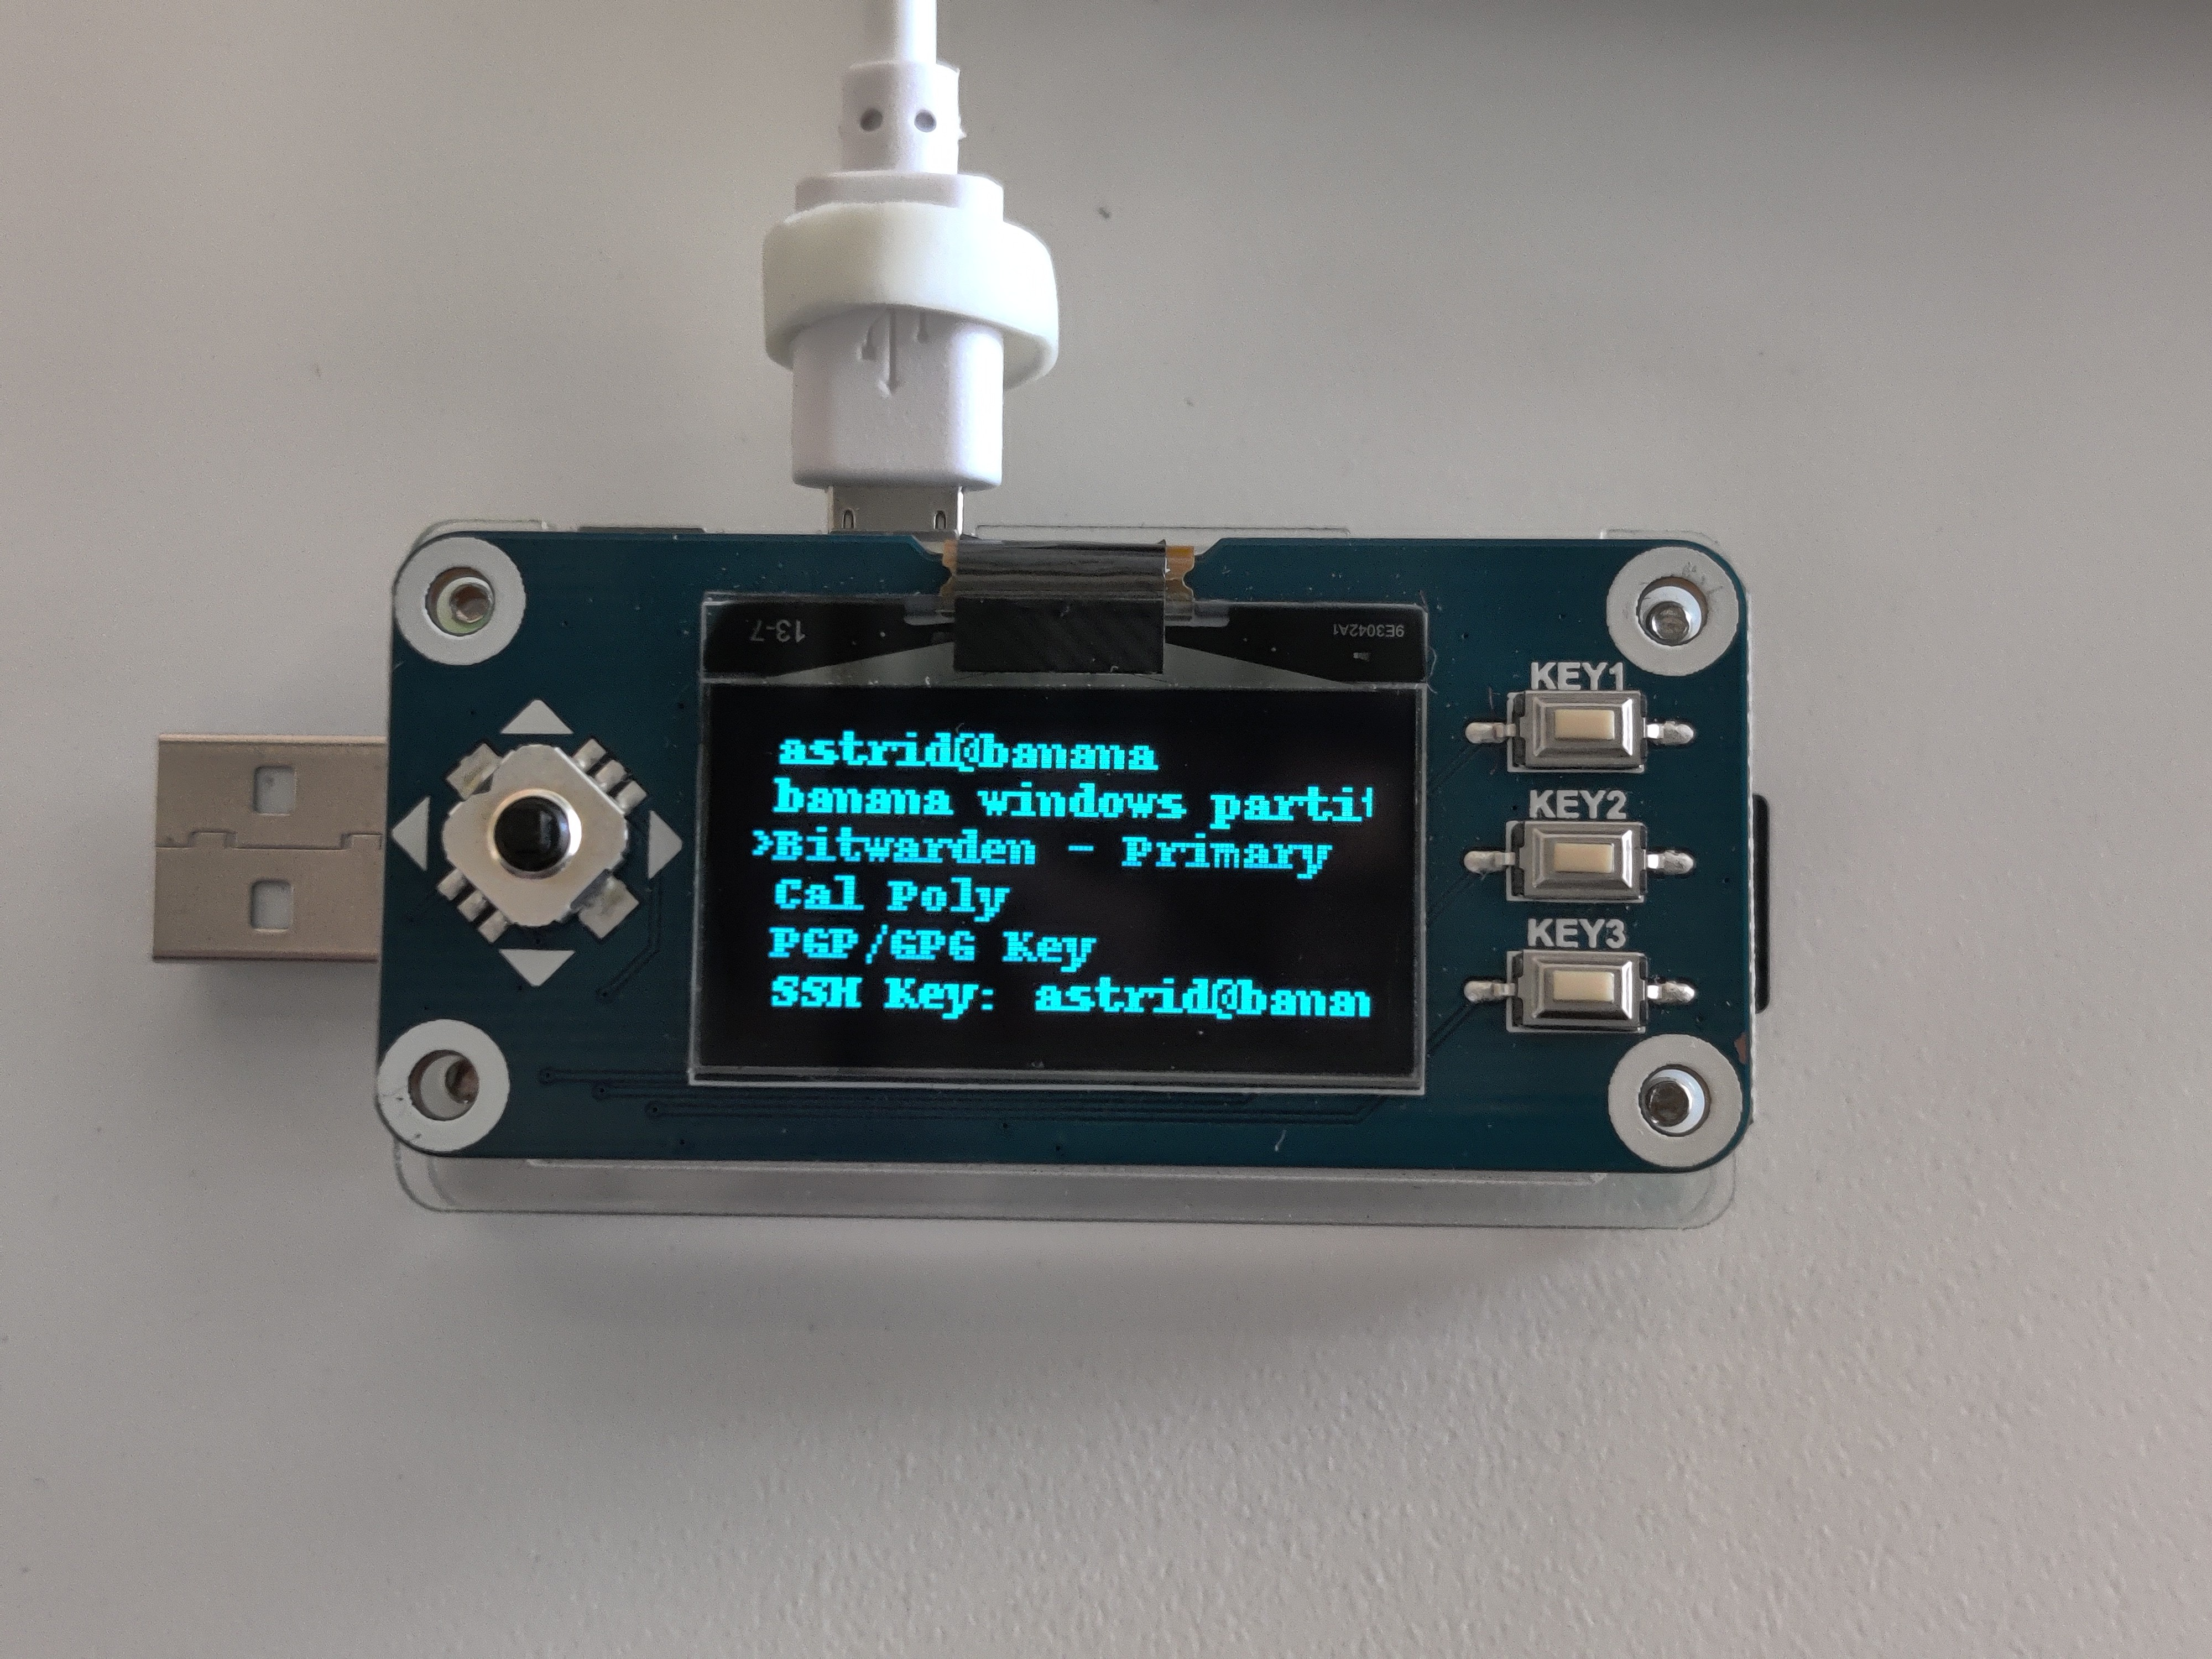
\includegraphics[width=10cm]{./unlocked.jpg}
    \caption{The Skeleton Stick in the password selection mode.}
    \label{fig:pwselect}
\end{figure}

\section{Design}

\subsection{Hardware}

This device is very cheap to produce. The total bill of required materials is listed below:

\begin{center}
\begin{tabular}{| l | r |}
    \hline
    \textbf{Item} & \textbf{Price} \\
    \hline
    \href{https://www.raspberrypi.com/products/raspberry-pi-zero/}{Raspberry Pi Zero} & \$5.00 \\
    \href{https://www.waveshare.com/1.3inch-oled-hat.htm}{Waveshare 1.3" OLED HAT} & \$11.99 \\
    \hline
    \textbf{Total} & \$16.99 \\
    \hline
\end{tabular}
\end{center}

Optional materials are listed below:

\begin{center}
\begin{tabular}{| l | r |}
    \hline
    \textbf{Item} & \textbf{Price} \\
    \hline
    \href{https://www.amazon.com/iUniker-Expansion-Breakout-Raspberry-Inserted/dp/B07NKNBZYG/}{Double-sided USB Dongle Attachment + Case} & \$11.99 \\
    \hline
    \textbf{Total} & \$11.99 \\
    \hline
\end{tabular}
\end{center}

Assembly instructions are included with these materials, so it is left as an exercise to the reader.

\subsection{Software}

\subsubsection{Pi Zero as a HID}

The Skeleton Stick runs on \href{https://www.raspberrypi.com/software/}{Raspberry Pi OS Lite Bullseye}. However, several modifications have been made to the OS to allow the Pi to support being a HID:\footnote{The method is borrowed from \url{https://www.isticktoit.net/?p=1383}}

\begin{itemize}
    \item In \texttt{/etc/modules}, we load the kernel modules \texttt{dwc2} and \texttt{libcomposite}.
    \item We set the device tree overlay to dwc2 in \texttt{/boot/config.txt}. This is done by appending \texttt{dtoverlay=dwc2} to that file.
\end{itemize}

Once that is done, a special script in the program is used to actually connect and initialize the device.

\subsubsection{Program and CLI}

The program is written in Python 3.9. It is an executable Python package with a convenient CLI. The same code runs on both the computer and the Skeleton Stick.

\subsubsection{SystemD Services}

On the Skeleton Stick, the program is started as a pair of SystemD services that runs after \texttt{basic.target}. One service initializes the USB gadget connection, and the other service starts the UI that displays on the OLED.

Unfortunately, the Pi Zero is a very weak device, so this program boots in approximately 60 seconds, making it somewhat impractical for daily use. In future versions, I may consider rewriting the program in a lower-level language like Rust, and possibly even substituting SystemD for my own init process.

\subsection{Encrypted Password File}

\subsubsection{Protocol}

\paragraph{Encryption} During the encryption phase, the user supplies a password $P$, composed of UTF-8-encoded joystick directions, a plaintext $M$ composed of an encoded list of password entries.

Each password entry is composed of a name and a password value. It is converted into a JSON string like so and then minified. Here is an example of how it may look, but non-minified:

\begin{verbatim}
[
    { "name": "Google Account", "password": "87sfdguhijs" },
    { "name": "Cal Poly Account", "password": "7sfuydsfg" },
    { "name": "ZFS Disk Key", "password": "78sfdguisjnkdg3" }
]
\end{verbatim}

Once Skeleton Stick receives the user input, it generates a random 32-byte salt $S$ and generates the symmetric key $K$ (kept secret) as follows:
$$K = \pbkdf(P, S, 300000)$$

To generate the ciphertext $C$ and generate message authentication code (MAC) $H$, we use AES in EAX mode. This requires generating a random 16-byte nonce $N$. We calculate $H$ and $C$ like so:
$$(C, H) = \aese_K(\pkcs7(M), N)$$

Then, we store $C, H, S, N$ on the disk.

\paragraph{Decryption} To decrypt the data on the Pi and re-derive $M$, we are given $C, H, S, N$ and the user-inputted $P$. We can essentially follow all these steps in reverse.

Generate $K$, also with
$$K = \pbkdf(P, S, 300000)$$

Then, decrypt and verify $M$ using MAC $H$:
$$M = \pkcs7^{-1}(\aesd_K(M, H, N))$$

\subsubsection{File Format}

Here, we describe the version 0 password file. Note that we will use Python-style byte strings.

A Skeleton Stick password file begins with byte string \verb$__SKELETONSTICK\n$ to act as a magic number, similar to how ELF files start with \verb$\x7fELF$ or how BMP files start with \texttt{BM}. Then, 4 bytes are used to store the version, which is simply \texttt{0x00000000}.

After that, its header is composed of several fields, seen in Figure \ref{fig:headerfmt}.

\begin{figure}
    \centering
    \begin{bytefield}{32}
        \bitheader[endianness=big]{31, 16, 15, 0} \\
        \wordbox{1}{$S$} \\
        \bitbox{16}{$N$} & 
        \bitbox{16}{$H$} \\
        \bitbox{4}{$|C|$}
    \end{bytefield}
    \caption{The byte field format of the password file header. Note that $|C|$ refers to the length of $C$.}
    \label{fig:headerfmt}
\end{figure}

The body following the header is simply the bytes of $C$, followed by the byte string \verb$\nEOF$ as an end of file marker.

This file format can be stored as a file on disk, but it is also designed to be written directly onto the beginning of a partition, to allow for future versions of Skeleton Stick to potentially operate at a lower level on the hardware by directly reading the disk.

\section{Security Analysis}

In general, all of the potential attacks on Skeleton Stick will require physical access, or control over the computers it's used on. When it's not under debugging, the Wi-Fi and Bluetooth chips will be disabled or removed completely (i.e. by using a Pi Zero instead of a Pi Zero W), so wireless access to the device is not possible.

As such, a simple mitigation to almost all possible attacks would be to simply ensure physical custody of the device at all times. The Skeleton Stick should be treated like a physical key to your house, because it is. However, if that fails, there are other mitigations that can be taken.

\subsection{Shoulder surfing}

When transcribing a password from a phone password manager onto a public computer, the password is displayed in plaintext on the phone, so people standing behind you can potentially steal the password that way. The Skeleton Stick completely eliminates that possibility by hiding the passwords and directly entering them into the device.

However, a noisy way for someone to recover a password from the Skeleton Stick could be to press the ``send'' button while the user is typing something in plaintext and the Skeleton Stick is decrypted. This can be prevented by re-encrypting the Skeleton Stick every time you finish using it.

\subsection{Keylogger attacks}

The Skeleton Stick does not prevent passwords from being stolen via keyloggers. The user would have to make sure that they aren't plugging the Skeleton Stick into a hardware keylogger between them and the computer, and that the computer they are plugging the Skeleton Stick into does not have a software keylogger, either.

\paragraph{Hardware keyloggers} Usually, USB hardware keyloggers can be slipped between a keyboard and the computer on a public terminal. However, because the user is \textit{physically} plugging the device into a USB port, they would likely either detect that USB keylogger or simply plug it into a different port. However, there is still risk from an attacker planting a hardware keylogger \textit{inside} the computer, perhaps between the USB port and the motherboard headers.

\paragraph{Software keyloggers} The Skeleton Stick would likely exhibit similar characteristics as if the user were to transcribe passwords from their phone app onto the keyboard. The software keylogger would be able to catch any passwords that the Skeleton Stick is sending to the computer, but so long as the user isn't using a software password manager on the computer, then only those passwords would be recorded.

Of course, if there \textit{is} a software keylogger, it is likely that the machine is also compromised in other ways, so the user should avoid entering passwords or doing sensitive activities on public computers in the first place.

\subsection{Cold boot attacks}

There is no unencrypted plaintext on disk, but the PIN and the plaintext \textit{does} exist in memory. The Raspberry Pi doesn't have secure hardware memory erasure, so it is vulnerable to a cold boot attack.

\subsubsection{Vulnerable states}

There are a couple of device states that could be vulnerable to a cold-boot attack.

\paragraph{PIN entry/Key derivation} This state refers to any point where the user is entering the PIN, or the hash function is being applied to the PIN. The PIN, or at least parts of it, would certainly be in memory.

A partial PIN would provide a lot of information for an attacker to perform a brute-force attack; a full PIN would allow the attacker to easily steal the passwords, if they get access to the password file (and since this is a physical attack, they most certainly will).

\paragraph{Passwords decrypted} The passwords have been decrypted and the user is selecting a password to enter. Obviously, the passwords would be in RAM at this point.

\paragraph{Passwords re-encrypted} The passwords were decrypted at one point, but the user has since re-encrypted the passwords.

Since the proof of concept program is written in Python, which is a high-level, garbage collected language, there is a chance that the plaintext has not yet been freed, or that it has been freed but not securely erased (i.e. by overwriting with random data or zeroes). 

\subsubsection{Performing the attack}

The form factor of the Pi Zero makes it extremely easy to perform a cold boot attack. It could be done as follows:

\begin{enumerate}
    \item Swipe the Skeleton Stick. This will likely disconnect the power supply, if it's not already disconnected.
    \item Swap out the SD card for a customized SD card that performs a memory dump.
    \item Power the Skeleton Stick back on, likely with a portable battery pack.
\end{enumerate}

However, the attacker would have to strategically select a time to swipe the stick.

\paragraph{While in active use} Suppose the attacker swipes when the user is actively using the device and it is in a vulnerable state. This would yield the highest probability of success by maximizing the chance of RAM remanence.

However, this would be a very noisy attack; likely, the attacker would be swapping out the SD and plugging in the portable battery pack while sprinting away from the user. Still, users should make sure that they have full custody of the stick during the entire time it's plugged in.

\paragraph{Shortly after unplugging} If the user unplugs the device in a vulnerable state, packs it away, and looks away, the attacker may be able to swipe it within seconds or minutes. However, the chance of RAM remanence would be lower, so the attack may be less successful.

\subsubsection{Mitigation: Maintain physical custody}

Once again, the cold boot attack and any physical attack will only work if the attacker is able to swipe it. If you keep it in your field of view at all times, and ensure it can't be swiped, the attacker can't do anything.

\subsubsection{Mitigation: Lock before unplugging}

If you can't maintain custody after packing it away, doing this will minimize the chance that vulnerable data remains in memory. Of course, the proof-of-concept program is written in Python, so this is not a guarantee, which brings us to the next potential mitigation.

\subsubsection{Potential Mitigation: Secure memory erasure}

Python does not have much in terms of primitive memory manipulation features. Thus, it may be useful to rewrite the program (or at least these more critical parts) in a lower-level language, like C, Assembly, or Rust, that can allow this secure erasure of the data in RAM.

However, this may not be enough, especially if the kernel reallocates the page or swaps it. Instead, it may be necessary to use a static portion of physical memory for these sentitive contents, so that they actually get overwritten physically.

\subsection{Offline attacks on the password file}

If an attacker gained offline access to the password file (perhaps by stealing the SD card and copying it off the disk), they would have access to the following information:

\begin{itemize}
    \item The nonce and MAC from EAX mode AES
    \item Ciphertext of the user's passwords
    \item Length of the user's passwords
    \item Key derivation function cost
\end{itemize}

The most efficient way to break this password file would likely be by going through all possible PINs and running it through the KDF under the known cost. So, the user would have to consider the convenience/security tradeoff when selecting a PIN and a KDF cost.

Since the alphabet is only 5 symbols, each additional symbol will only yield $\log_2(5) = 2.32$ bits of entropy. If the recommended password entropy is $77$ bits, then the PIN would need to be $34$ symbols long! That may be long, but it is potentially memorable.

Besides lengthening the PIN, there are a few other ways to improve its security.

\subsubsection{Mitigation: Key stretching}

Using a larger cost could increase the effective entropy by a constant amount. For example, using a cost that is 3 times higher would increase the effective entropy of all passwords by a constant $\log_2(3) = 1.58$ bits. However, this will also mean that the length of the decryption step (which is already dominated by the key derivation function) takes 3 times longer. It already takes a very long time, since the Pi Zero has such a weak processor, so this can only have a limited benefit before it becomes highly inconvenient.

\subsubsection{Potential Mitigation: Expanding the alphabet}

The PIN entry interface is pretty maximally utilized, so unless we create custom hardware, it's simply not possible to include more buttons. However, we could encode additional information into our button presses, such as by looking at the time domain.

Note that all of these features would require additional code, so they are not actually implemented. However, they are listed here as possible future improvements.

\paragraph{Long/Short Presses} If we record inputted symbols as short presses or long presses, this increases our alphabet by a factor of 2. We could render short as lowercase and long as uppercase. For example, \texttt{short center} would be \texttt{c} and \texttt{long center} would be \texttt{C}.

\paragraph{"Shift" Key} Currently, clear and backspace are on two different buttons. If we merge the clear and backspace into one button (i.e. short for backspace, long for clear), we could free up an additional button to use as a ``shift'' key.

\begin{CJK*}{UTF8}{gbsn}
When a joystick direction is pressed, the state of the shift key would be recorded with it as well, and the keys would write a different character; instead of \texttt{UDLRC}, it could be \texttt{SXZYQ}. \footnote{In Chinese, 上下左右前, pronounced \textit{shàng xià zuǒ yòu qián}, means ``up, down, left, right, front.'' 中 (zhōng) could not be used because 左 already occupies \texttt{Z}.}
\end{CJK*}

For example, \texttt{short up} could be rendered as \texttt{u}, but \texttt{shift + short up} would be rendered as \texttt{s}, and \texttt{shift + long up} would be rendered as \texttt{S}. This would increase our alphabet by a factor of 2.

\paragraph{Space characters} We could even record the time between inputted symbols as short or long pauses to read in "space" characters. For example, if the user inputs something like \texttt{<short up> <long right> <short center>}, waits, then enters \texttt{<shift + long left> <short right>}, this would be rendered as \texttt{uRc Ps}. Though this only increases our alphabet by 1 symbol, since spaces can't be shifted, spaces can make the password more memorable, and make it easier for the user to increase the password length.

\paragraph{Adding it all together} Our full alphabet could go from the 5-symbol \texttt{UDLRC} to the 21-symbol \texttt{uUdDlLrRcCsSxXzZyYqQ} plus a space. This has an entropy of $4.39$ bits, which nearly doubles our per-symbol password entropy by combining all of these techniques! This way, to reach $77$ bits, we only need a $18$ symbol PIN, which is a lot easier to memorize.

However, it must be noted that doing so will make the user interface somewhat more difficult to use. Also, the user might not end up using features such as the shift key. Once again, there is the eternal tradeoff between convenience and security.

\section{Conclusion}

The Skeleton Stick is an effective device that fills in the gap between a password managers and low-level login interfaces. It is not meant as a replacement for software password managers, but as an additional part in a comprehensive password security solution.

When using the Skeleton Stick, users should take as many precautions as possible to avoid keylogger attacks and physical access attacks, primarily ensuring that the device is always in their physical custody.

What I have created is a proof of concept. However, there are many ways for the device to be improved in the future, both in terms of security features (such as expanding the alphabet) and in terms of performance (such as reducing the boot time).

\end{document}


